\scanpage{33}

\uline{Fermés de Lefschetz-Grauert}

1) Définitions, remarques

\uline{Déf} Soit $X$ un préschéma loc noeth, $Y$ une partie
fermée, $n$ un entier. On dit que $Y$ a la propriété
$(LG)_n$ dans $X$ \deleted{\unsure{propriété} \unsure{d'ordre} $n$},
si pour $\forall$ $F$ loc. libre sur $X$,
\[
(\alpha)\qquad H^i(X,F)\longrightarrow H^i(X_{/Y},F_{/Y})
\deleted{\unsure{\text{est}}}
\]
est bijectif pour $i\leq n$, \inserted{et injectif pour $i=n+1$.}

\margin{Inutile}

On dit que $Y$ a la propriété $LG$ \inserted{faible en $X$} si
\inserted{pour tout $F$ loc. libre sur $X$,}
\deleted{elle a la propriété $(LG)_0$}
\[
H^0(X,F)\xrightarrow{\sim}H^0(X_{/Y},F_{/Y})
\]
[i.e. $F\longmapsto F_{/Y}$ est pl. fid. des Mod. loc. libres
sur $X$ \unsure{dans ceux} sur $X_{/Y}$]

On dit que $Y$ a la propriété $LG$ \deleted{dans $X$} pour
tt voisinage ouvert $U$ de $Y$, \deleted{$Y$}
\inserted{\unsure{la dite} propriété $LG$ faible en $U$.}
\deleted{\unsure{si}} $Y$ a la propriété $LG$,
\inserted{\deleted{\unsure{définie}} si elle a la propriété $LG$,}
et si de plus \deleted{pour}
$\forall$ $\unsure{\mathfrak F|\mathcal F}$ loc. libre sur $X_{/Y}$,
\deleted{\unsure{il}} est isom. à un faisceau de la forme
$F_{/Y}$, avec $F$ loc libre sur un voisinage ouvert $U$ de $Y$.

\margin{\figure{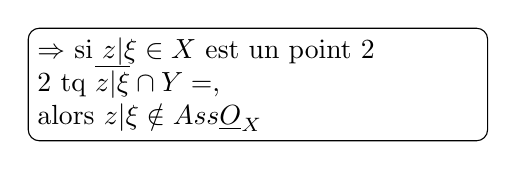
\begin{tikzpicture}
\node[draw,rounded corners,align=left,text width=5.6cm] {$\Rightarrow$ si $\unsure{z|\xi}\in X$ est un
\deleted{\unsure{point} \illegible{2}}\newline
\deleted{\illegible{2}}
\unsure{tq} $\overline{\unsure{z|\xi}}\cap Y=\varnothing$,\newline
alors $\unsure{z|\xi}\notin\operatorname{Ass}\underline O_X$};
\end{tikzpicture}}}

\margin{Question : $(\unsure{LG})$ \deleted{\unsure{?}}
implique que \unsure{d'alors} \deleted{\unsure{pour tout}}
$x\in X$ tq $\bar x\cap Y=\varnothing$, ???
$\operatorname{prof} O_{X,x}\geq2$}

Donc la propriété $LG$ stricte signifie que les foncteurs
$\mathcal L(U)\mathbin{-}\mathcal L(V)$
[$\forall U\supset V\supset Y$] sont pleinement fidèles, et
\diagram{\begin{tikzcd}[column sep=small,row sep=large]
& \displaystyle\mathop{\mathrm{Lim}}_{\substack{\longrightarrow\\U\supset Y}}
  \arrow[dl,leftrightarrow] &
\underbrace{\mathcal L(U)}_{\substack{\text{Catégorie des}\\\text{Modules loc}\\\text{libres sur }U}}
  \arrow[r] & \mathcal L(X_{/Y}) \\
\substack{\text{``\unsure{Précaution}'' de}\\\text{catégories}} &&&
\end{tikzcd}}
est une équivalence de catégories.

\margin{\figure{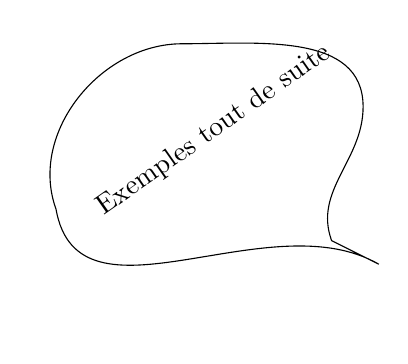
\begin{tikzpicture}
\node[rotate=35] (t) at (0,0) {\uline{Exemples \unsure{tout} de suite}};
\draw (-2,-1) to[out=110,in=180] (-.4,1.1)
to[out=0,in=90] (1.9,.3) to[out=-90,in=110] (1.5,-1.4)
--(2.1,-1.7) to[out=150,in=-80] (-2,-1);
\end{tikzpicture}}}

\margin{32}
